\chapter{Defining some concepts and redifining the variables} 
\section{Voices, parts and strata}\label{section:parts-and-strata}
Before we start this section, we need to look at some vocabulary to make sure we understand what we are discussing. The most important definition (and distinction) we will introduce is the definition of the terms \textit{part} and \textit{stratum}. The need for these definitions arises from the increasing complexity of the rules of counterpoint when it is generalised to three voices. Indeed, the rules are no longer (as we shall see later) concerned solely with counterpoint and its cantus firmus, but also with new concepts, such as that referred to by Fux as 'the lowest voice'. As the term 'voice' is too generic (it is used in Fux's text to describe notions as different as counterpoint, cantus firmus, voice range and the so called 'lowest voice'), we need to create a precise vocabulary that is different from the word 'voice' to talk about these new concepts. 

With this in mind, let's explain what 'parts' and 'strata' are. Each of these two concepts is a type of voice, which means that in a composition with $n$ voices, there will also be $n$ parts and $n$ strata.

The \textbf{parts} correspond to what a given individual sing. They correspond to a staff (each staff corresponds to one part). The term 'part' is the same as that used by Fux in his work. The \cf, like each of the counterpoints, are parts. The parts are usually called "bass", "tenor", "alto" and "soprano" (and even more).

As for the \textbf{strata}, they are defined like this: a stratum delineates discrete layers or levels of pitches at any given moment in the composition. It denotes a vertical alignment of simultaneous notes and organizes them into distinct strata. By definition, the lowest stratum encompasses the lowest sounding notes, the highest stratum comprises the highest sounding notes, and intermediary strata represent pitch levels in between.
This concept is very helpful in identifying and categorising the vertical placement of pitches, creating distinct categories of sound within the overall texture of the counterpoint composition. It provides a way of analysing and understanding the distribution of pitches across different parts, allowing more complex rules to be established: for example, it would now be possible to establish a rule between the notes of the cantus firmus and the highest sounding notes (no matter which part they come from). The full potential of strata lies in harmonic rules, but as we shall see, some melodic rules are also related to it.

\begin{minipage}{0.6\textwidth}
    The term stratum was chosen in this context for its visual impact. In geology, a stratum "is a rock layer with a lithology (texture, colour, grain size, composition, fossils, etc.) different from the adjacent ones", see figure \ref{fig:geological-strata}.
    \end{minipage}
    \hfill
    \begin{minipage}{0.3\textwidth}
      \centering
      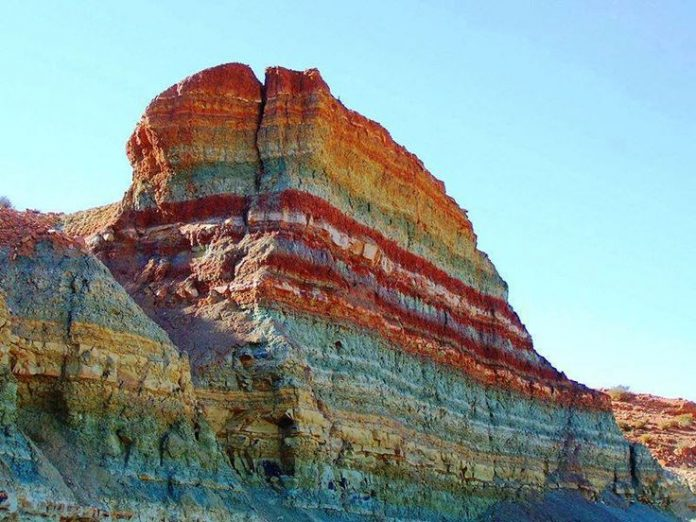
\includegraphics[width=\textwidth]{Images/rainbow-sediment.jpg}
      \captionof{figure}{Geological strata, for the illustration}
      \label{fig:geological-strata}
\end{minipage}
\vspace{.5cm}

The choice of calling the stratum corresponding to the smallest pitches the 'lowest' stratum rather than 'bass' (like Fux does) is deliberate: 'bass' is also the name of a range of voices (on a par with soprano and alto, for example), and there is already enough complexity in all the terminology to add even further ambiguity.

\paragraph{}
These new terms (parts and strata) are used where the distinction between the concepts is important. Where the distinction is not important, the more general term 'voice' is used to reduce the complexity of reading. In this case, the 'voice' could refer to both a layer and a part.

Since a picture is worth a thousand words, Figure \ref{fig:lowest} illustrates the difference between parts (the blue lines) and strata (the red and orange lines). The lowest stratum is shown in its own colour (red) because it is the most meaningfull stratum, and it will be particularly important later on.

\begin{figure}[h]
  \centering
  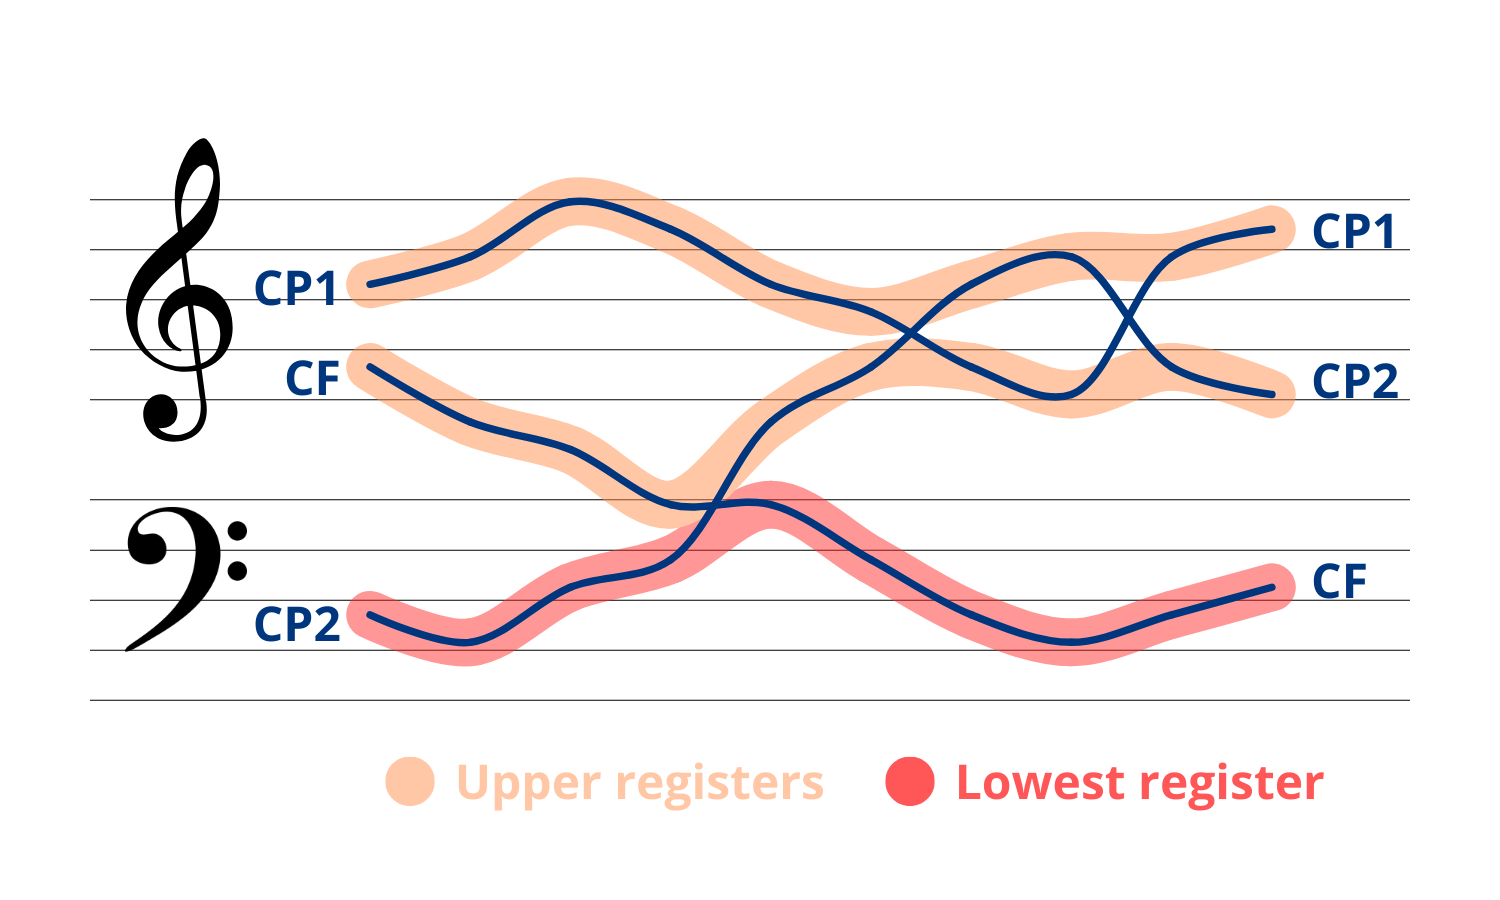
\includegraphics[width=1\textwidth]{Images/lowest.png}
  \caption{Parts and strata in a three voice composition}
  \label{fig:lowest}
\end{figure}


Here is also the mathematical representation for the notes of the lowest stratum (written $N^{\lambda}$, see section \ref{section:changes induced} for the notations):
\begin{equation}
    \forall i \in [0, 3], \quad \forall j \in [0, m-1): N^{\lambda}[i,j] = \text{min} (N^{cf}[i,j], N^{cp_1}[i,j], N^{cp_2}[i,j])
\end{equation}

Of the first upper stratum, or medium stratum (written $N^{u_1}$, see section \ref{section:changes induced} for the notations):
\begin{equation}
    \forall i \in [0, 3], \quad \forall j \in [0, m-1): N^{\lambda}[i,j] = \text{med} (N^{cf}[i,j], N^{cp_1}[i,j], N^{cp_2}[i,j])
\end{equation}

And of the second upper stratum, or uppest stratum (written $N^{u_2}$, see section \ref{section:changes induced} for the notations):
\begin{equation}
    \forall i \in [0, 3], \quad \forall j \in [0, m-1): N^{\lambda}[i,j] = \text{max} (N^{cf}[i,j], N^{cp_1}[i,j], N^{cp_2}[i,j])
\end{equation}

\section{Exploring the interaction of the parts with the lowest stratum}

One of the major differences between the composition of two voices (i.e., one \cf and one counterpoint) and the generalisation to three voices (i.e., one \cf and two counterpoints) is that the rules no longer necessarily apply between the counterpoints and the \cf. If we go back to the rules for two voices, we see that each of them applied between the single counterpoint and the \cf. For example, when it was stated that each interval must be consonant, this referred to the interval between the counterpoint and the \cf.
On the other hand, in his second part (where he describes the rules for composing in three voices), Fux explains that the rules are not necessarily to be observed between each of the counterpoints and the \cf, but rather between "each of the voices and the lowest voice" (i.e. the lowest stata). Again, if we take the example of the need for consonance between the voices, consonance will be required in the intervals between the notes of any voice and those of the lowest voice (whether or not the latter is the \cf).
Fux approaches the concept of lowest stratum without ever stating it clearly, mentioning for example that the lowest voice can change (sometimes the bass is the lowest voice, sometimes the tenor, ...), and that at any given moment the lowest voice should be considered. In other words, Fux says that the rules apply between the parts and the lowest stratum.

\paragraph{}
One might be tempted to conclude that three-part composition breaks completely with two-part composition, but that would be too hasty a conclusion. Indeed, on closer inspection, the way the rules worked in two-part composition (from counterpoint to \textit{cantus firmus}) is just one particular case of this new vision of things. In two-part composition, too, the rules apply between the parts and the lowest stratum. But of course, since there were only two voices, the lowest stratum was either counterpoint or cantus firmus. This means that when links were established between the upper part and the lowest stratum, links were also established between the counterpoint and the cantus firmus. Considering the rules as being established between the counterpoint and the \cf was just a simplification of reality, although it was perfectly correct. We were therefore considering a convenient particular case, and not the general case. Please note that when we talk about "applying constraints from voice A to voice B", it is clear that the constraints are bidirectional and that they also apply from voice B to voice A. What is shown here is rather the philosophy behind the application of these constraints, and the reasons why they were imposed.

The particular case happening when composing with two parts is illustrated in figures \ref{fig:cp2cf-2v} and \ref{fig:p2l-2v}. As we can see on those pseudo-compositions, it does not change anything to apply the constraints from the counterpoints to the \cf or from the parts to the lowest stratum.

\vspace{.5cm}
\begin{minipage}{0.46\textwidth}
    \centering
    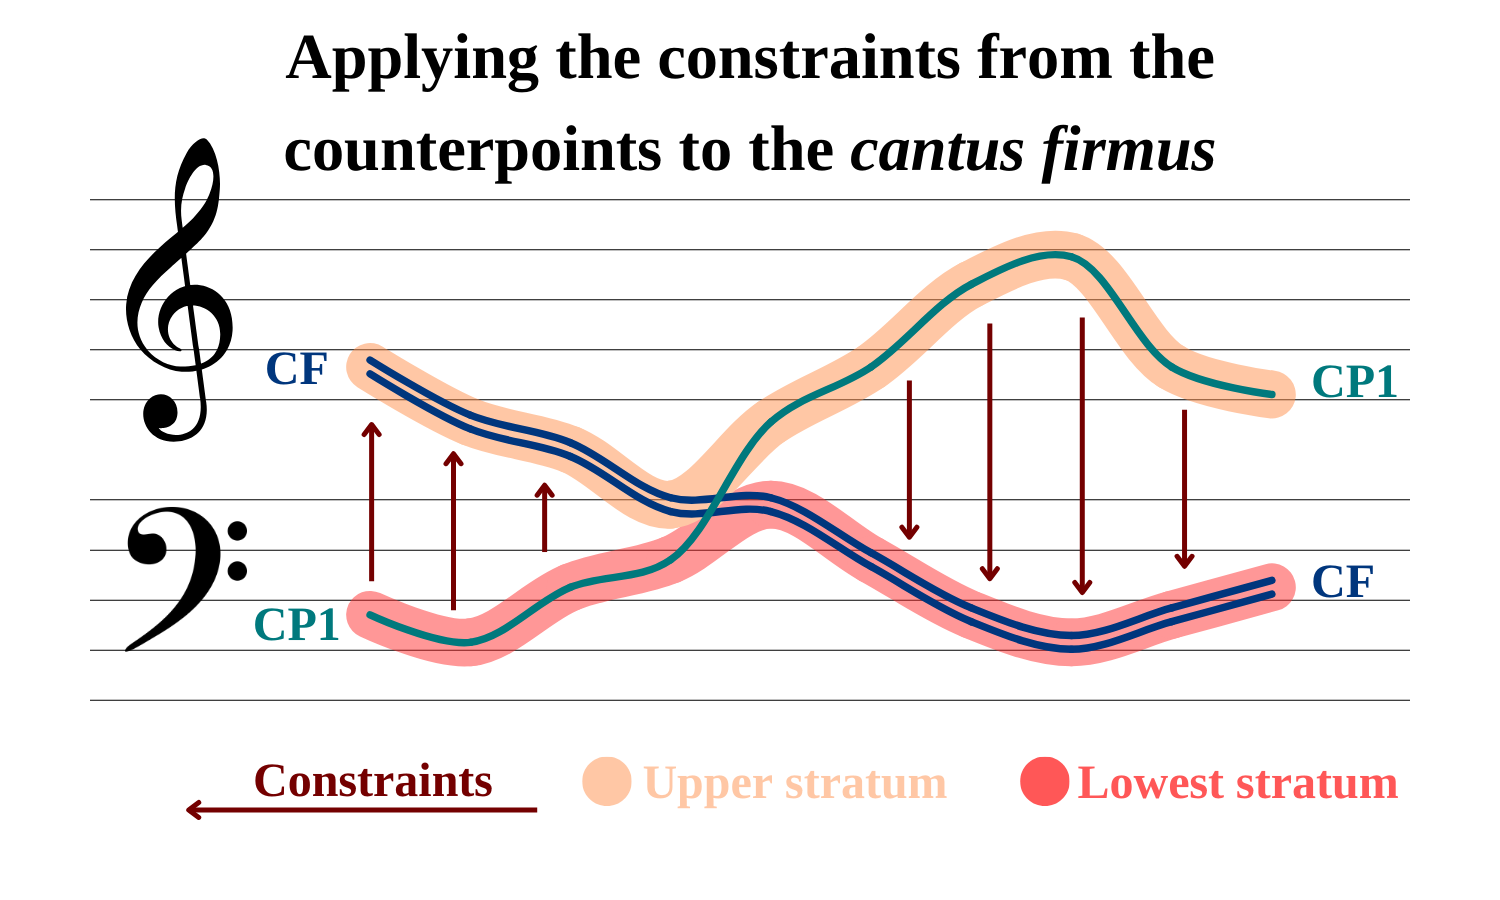
\includegraphics[width=\textwidth]{Images/cp2cf-2v.png}
    \captionof{figure}{Applying the constraints from the ctp. to the \cf}
    \label{fig:cp2cf-2v}
    \end{minipage}
    \hfill
    \begin{minipage}{0.46\textwidth}
      \centering
      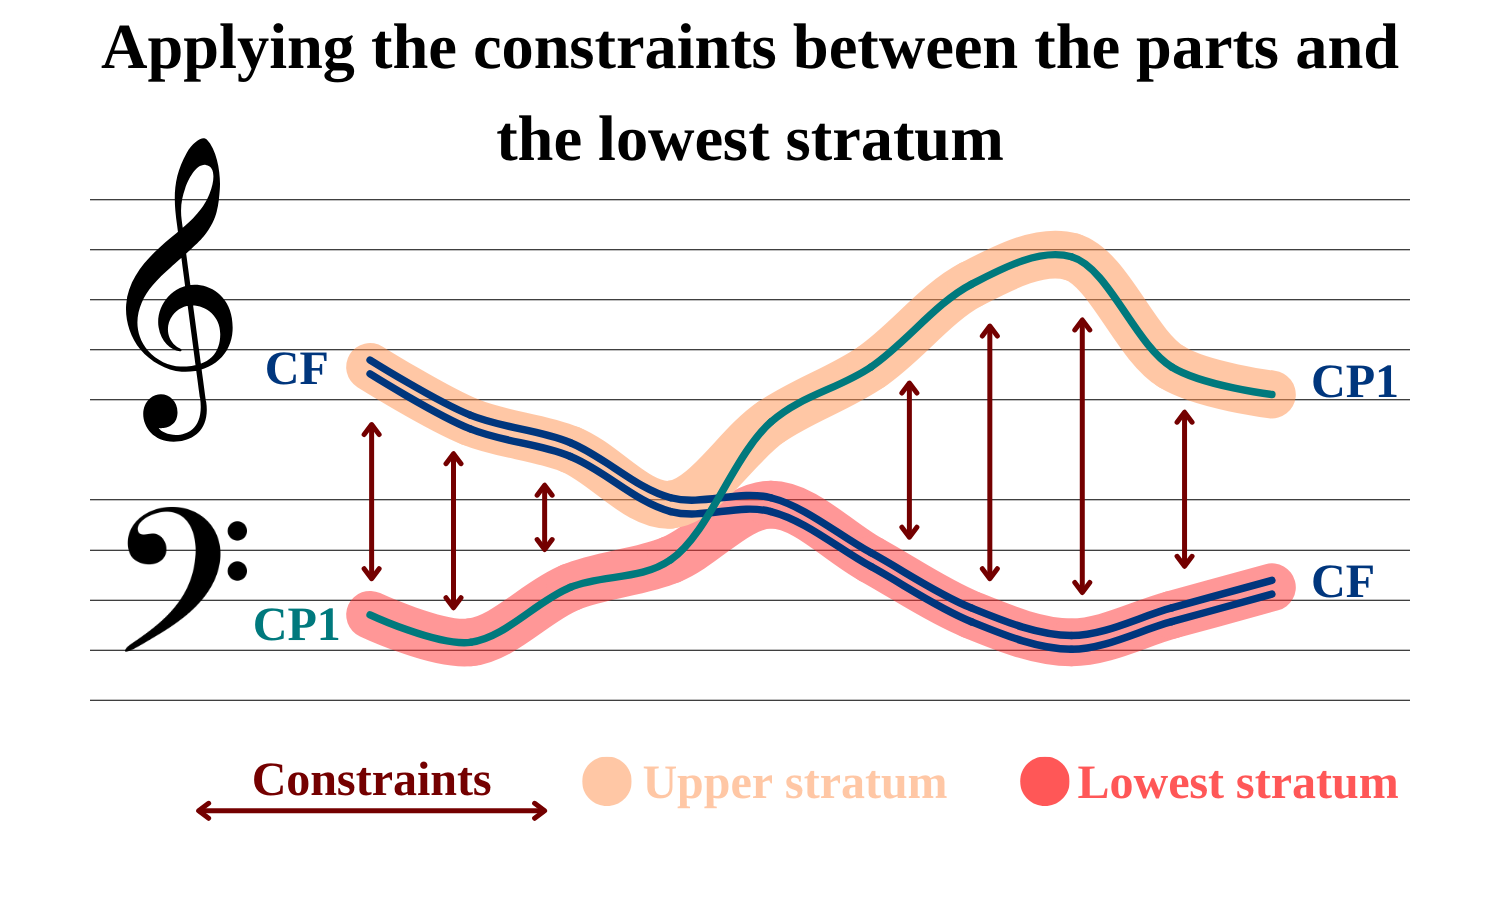
\includegraphics[width=\textwidth]{Images/p2l-2v.png}
      \captionof{figure}{Applying the constraints from the parts to the lowest stratum}
      \label{fig:p2l-2v}
\end{minipage}
\vspace{.5cm}

However, when it comes to generalising the composition of counterpoint for three voices, it is no longer possible to follow the same simplification. We are now forced to set our rules between the parts and the lowest stratum, and no longer between the counterpoints and the \cfdot On figures \ref{fig:cp2cf-3v} and \ref{fig:p2l-3v}, it is made clear that establishing the rules from the counterpoints to the \cf is really different than applying them from the various parts to the lowest stratum. In those figures, the parts don't cross and therefore match perfectly with the strata, hence the constraints are always applied to the same counterpoint. This was made for the sake of intellegibility of the graphs, but it is obviously possible that the parts cross and that the "target" of the constraints is not always the same counterpoint.

\vspace{.5cm}
\begin{minipage}{0.46\textwidth}
    \centering
    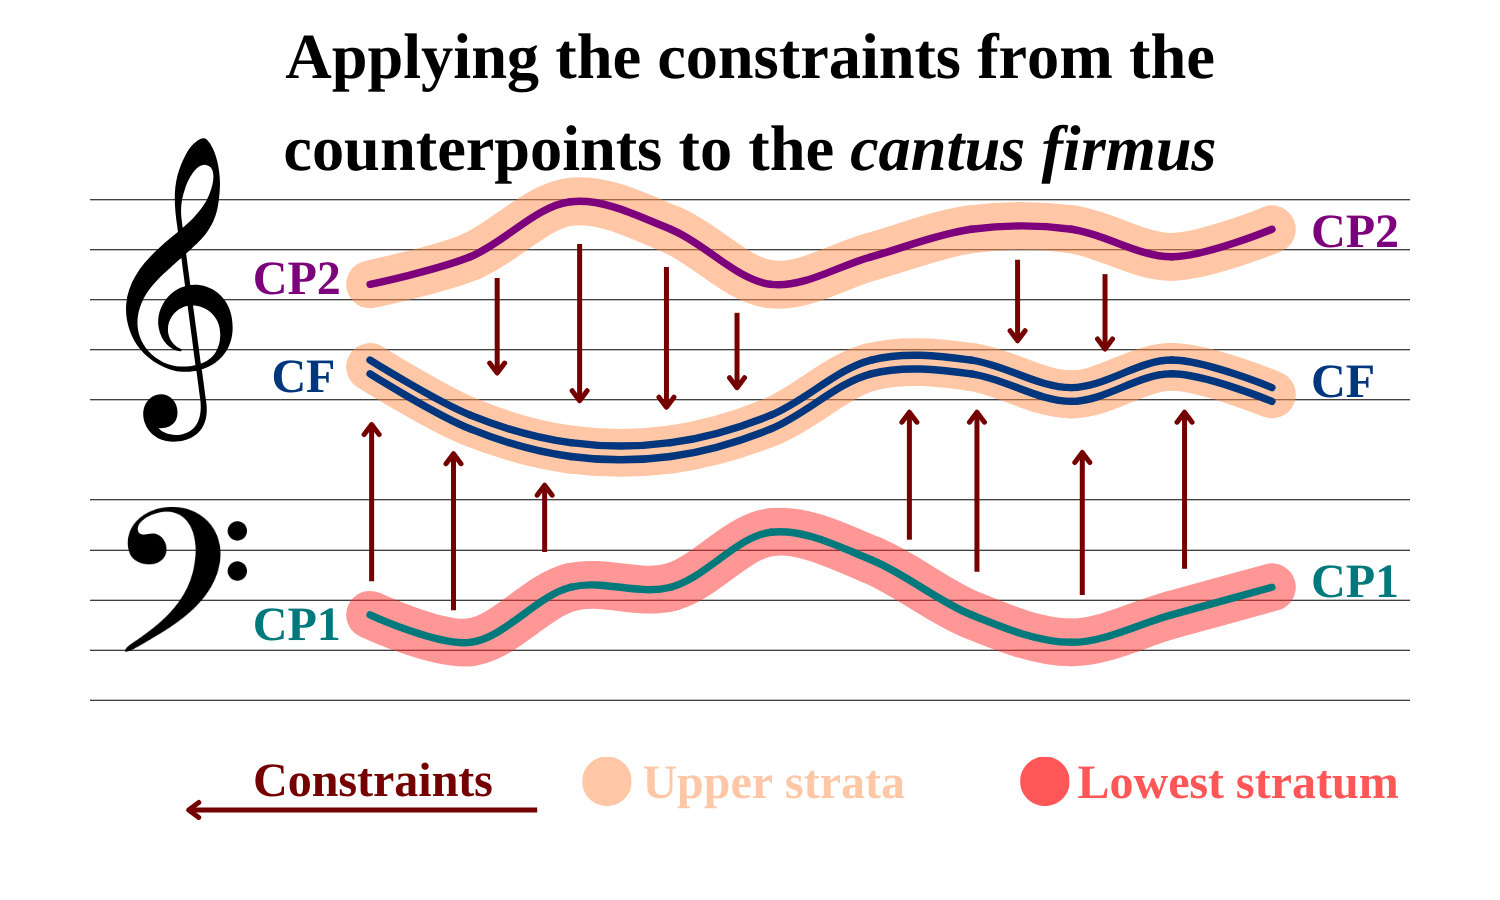
\includegraphics[width=\textwidth]{Images/cp2cf-3v.png}
    \captionof{figure}{Applying the constraints from the ctp. to the \cf}
    \label{fig:cp2cf-3v}
    \end{minipage}
    \hfill
    \begin{minipage}{0.46\textwidth}
      \centering
      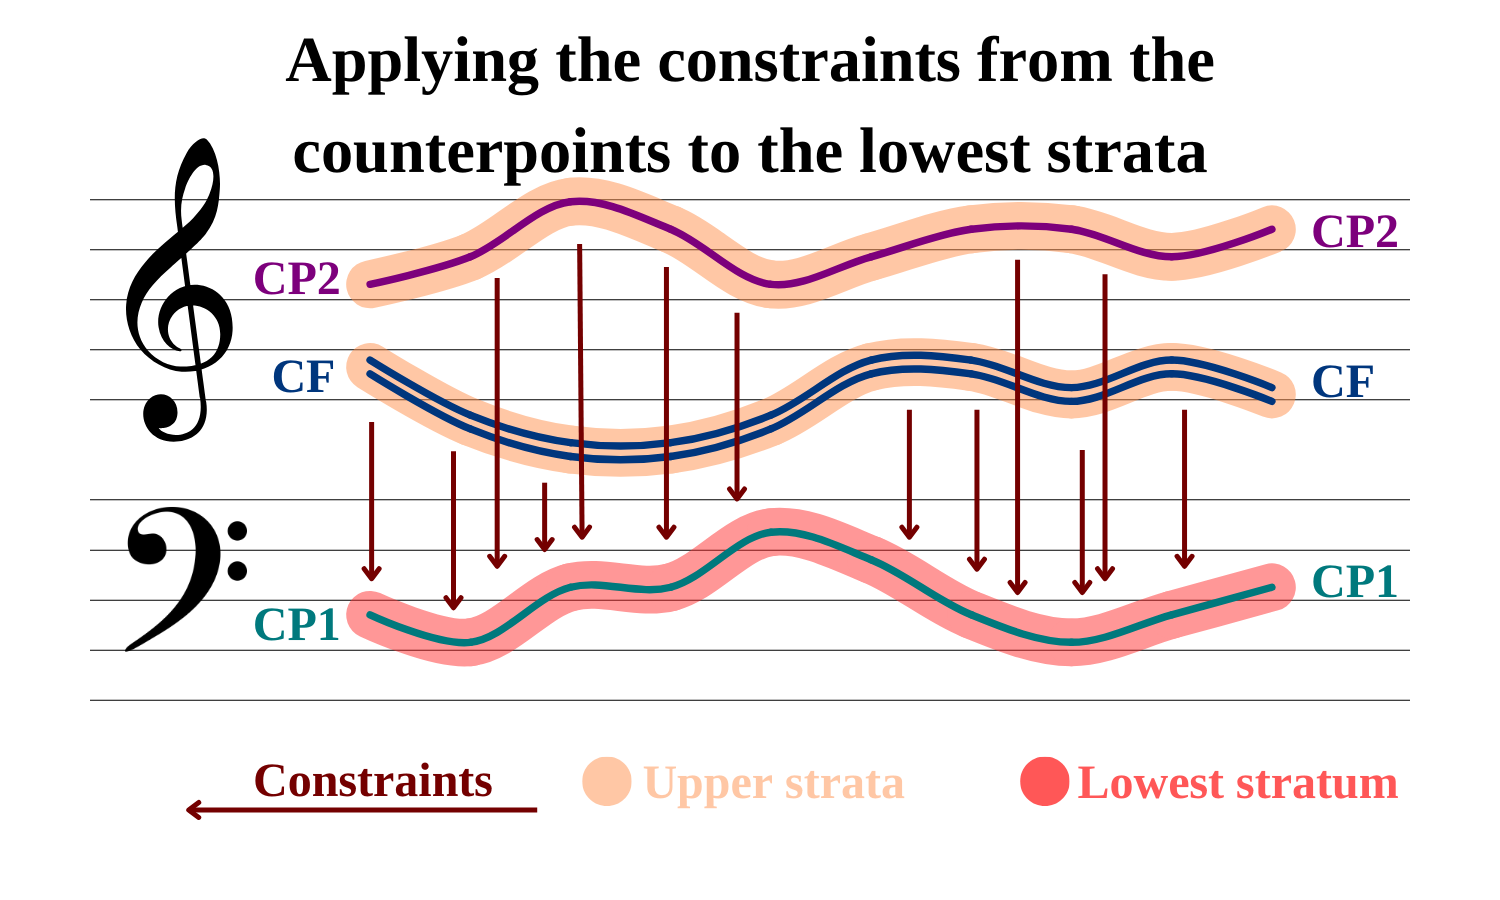
\includegraphics[width=\textwidth]{Images/p2l-3v.png}
      \captionof{figure}{Applying the constraints from the parts to the lowest stratum}
      \label{fig:p2l-3v}
\end{minipage}
\vspace{.5cm}

It is, of course, possible for the \cf to be equal to the lowest stratum all along, in which case nothing changes from the perspective we had when composing for two voices. In this particular case, by applying the rules with respect to the \cf, we would find ourselves de facto applying the rules with respect to the lowest stratum (and we would be back to the situation described above, see figures \ref{fig:cp2cf-3v} and \ref{fig:p2l-3v}, only that there is now one more part). It is when the \cf pitches are higher up than those of the counterpoints that considering the lowest stratum consideration becomes necessary.

\paragraph{}
A very important detail, and perhaps the biggest change brought about by this paradigm shift, is that the \cf now becomes a counterpoint like any other, with the difference that its notes are already fixed. This means that we will treat the \cf as a first species counterpoint (since it is always made up of whole notes), and that we will have to calculate its intervals, movements and costs, as we have already done with 'normal' counterpoints.

A second point to bear in mind, and not the least, is that all this does not mean that \textit{all} the rules are established between the parts and the lowest stratum. Certain rules will continue to apply between the different parts, regardless of whether they are high, low or intermediate.

\section{Changes induced in the variables} \label{section:changes induced}


Many changes have been induced as a result of the three part generalisation. In two part composition, it was obvious that the harmonic intervals array was describing the intervals between the \cf and the only counterpoint, it was obvious that the motions were those of the only counterpoint, and so it goes for all the variables. When writing a three part composition, we are dealing with many possibilities when speaking about "intervals" or motions. Intervals between which voices? Motions of which counterpoint? To tackle this, each variable is now related to a voice.

When written in the exponent of a variable, $cf$ means that the variable is related to the \cf. $cp_1$ means that the variable is about the first counterpoint and $cp_2$ means that the variable is about the second \cp.

When a variable is about the lowest stratum, its exponent is \textit{$\lambda$} (for \textit{l}owest; a $\lambda$ was chosen for this notation because it is much easier to read than a simple \textit{l}). The top voices are denoted \textit{u$_1$} and \textit{u$_2$} (for "\textit{u}pper").

When a variable is not explicitely linked to a part, it means that it is implicitely meant that the relation expressed for it is true for all the \textit{parts}. In other words, if variable X is written without an exponent, it means $\forall v \in \{cf, cp_1, cp_2\}: X^v$.

For example, the notation H$^{cp_1}$ corresponds to the variable representing the harmonic intervals of the first counterpoint, whereas H$^{cf}$ are the harmonic intervals of the bass (see section \ref{subsection:modified_variables} what this actually means). If only H is written, then the equation in which H is located holds true for any possible \textit{part} (and not necessary stratum). The harmonic arrays of the second upper stratum (the uppermost one) are written H$^{u_2}$.


This change applies to all variables (namely H, M, P, IsCfB, IsCons, and N (formerly cp)) and to all costs with the exception of $\mathcal{C}$ (the cost factors) and $\tau$ (the total cost). The two latter ones stay global and are not duplicated.

\subsection{Added variables}
\vspace{.5cm} \noindent \textbf{$\Lambda$} \hspace{.cm} \texttt{is-lowest} \label{is-lowest}

This boolean array of size $m$ reifies if the considered part is the lowest one. Its notation was chosen as it is the uppercase of $\lambda$ (the lowest stratum). It only takes into consideration the first note of every measure. The reason for this is that when all the rules were given according to the \cf, they were always based on the first beat of each measure (which is logical, as the \cf has no notes on the other beats). Given that the rules should work exactly the same way, they are only considering the first beat of the lowest stratum.
It is also worth to be noted that only one of the parts can be the lowest stratum at the time. This does not mean that two parts cannot equal the lowest stratum at the same time, they can. It means that only one of those two is going to be considered to \textit{be} the lowest stratum (and the other one will be the intermediate stratum). This is needed in order for motions to work well.

Here is the mathematical definition of the $\Lambda$ array:
\begin{equation}
\begin{aligned}
&\forall j \in [0, m-1) \colon  \\
&\Lambda^{cf}[j] := (N^{cf}[0,j] = N^\lambda[0,j])\\
&\Lambda^{cp_1}[j] := ((N^{cp_1}[0,j] = N^\lambda[0,j]) \land \neg \Lambda^{cf}[j])\\
&\Lambda^{cp_2}[j] := (\neg \Lambda^{cf} \land \neg \Lambda^{cp_1})
\end{aligned}
\end{equation}

In practice, there is only a \texttt{is-not-bass} array in the code (which is then equal to $\neg \Lambda$), as it is almost always more useful to know if a part is \textit{not} the lowest stratum than knowing if it is the lowest one. 


\subsection{Modified variables} \label{subsection:modified_variables}
Given that the majority of the rules now apply between parts and the lowest stratum, the meaning of the variables has been modified to adapt to this reality. 

\vspace{.5cm} \noindent \textbf{N} \hspace{.2cm} \texttt{notes} 

We changed the name of former \texttt{cp} array and renamed it to \texttt{N} (for notes), for the sake of clarity. As we have now three of those arrays (one for the first counterpoint, one for the second counterpoint, and even one for the \cf), it needed a less ambiguous name than the one it had before.


\vspace{.5cm} \noindent \textbf{H}$_{(abs)}^{v_1-v_2}$ \hspace{.2cm} \texttt{h-intervals}\hspace{.2cm} \texttt{h-intervals-abs}\hspace{.2cm} \texttt{h-intervals-to-cf}\hspace{.2cm} \texttt{h-intervals-cp1-to-cp2}

The way in which this variable works remains much the same, i.e. it represents the interval between one voice and another. This definition has been extended to include intervals other than that between the counterpoint and the \cf. Thus, H$^{v1-v2}$ represents the intervals between the $i$th beat of voice $v_1$ and the \textit{first} beat of voice $v_2$. By default, H$^{v_1}$ represents the intervals between the voice $v_1$ and the lowest stratum, so $H^{v_1} := H^{v_1-\lambda}$.

Here is a generalisation of the previous rule, matching to the current definition of the harmonic intervals array:
\begin{equation}
\begin{aligned}
    &\forall i \in \mathcal{B}, \quad \forall j \in [0, m) \quad \forall v_1, v_2 \in \{cf, cp_1, cp_2\}, v_1 \neq v_2:\\
    &H_{abs}^{v_1-v_2}[i, j] = \left|N^{v_1}[i, j] - N^{v_2}[0,j]\right|\\
    &H^{v_1-v_2}[i, j] = H_{abs}[i, j]\ \text{mod}\ 12\\
    &\text{where } H_{abs}[i, j] \in [0, 127], H[i, j] \in [0, 11]
\end{aligned}
\end{equation}


\vspace{.5cm}
\noindent \textbf{P} \hspace*{.2cm} \texttt{motions}

Motions are now calculated according to the movements of the lowest stratum. The problem here is that if a part is also the lowest stratum, we end up calculating the motion between a part and itself. This inevitably leads to direct motions being calculated, because a part is always moving in the same direction as itself. To solve this problem, the motions of a part are now equal to -1 when the part is also the lowest stratum (denoted $\Lambda$, see section \ref{is-lowest}). 
\begin{equation}
\begin{aligned}
&\forall v \in \{cf, cp_1, cp_2\}, \quad \forall x \in \{1, 2\}, \quad \forall i \in B, \quad \forall j \in [0, m - 1),\quad x := b - i\\
    P^{v}[i,j]& = \,  
    \begin{cases}
        -1 & \text{if } \Lambda^{v} \\
        0 & \text{if } \neg \Lambda^{v} \land ((M_{brut}^{x, v}[i, j] > 0 > M^{\lambda}_{brut}[j]) \vee\, (M_{brut}^{x, v}[i, j] < 0 < M^{\lambda}_{brut}[j])) \\
        1 & \text{if } \neg \Lambda^{v} \land (M_{brut}^{x, v}[i, j] = 0  \oplus M^{\lambda}_{brut}[j]=0) \\
        2 & \text{if } \neg \Lambda^{v} \land ((M_{brut}^{x, v}[i, j] > 0 \land M^{\lambda}_{brut}[j] > 0) \vee\, (M_{brut}^{x, v}[i, j] < 0 \land M^{\lambda}_{brut}[j] <0))
    \end{cases}
\end{aligned}
\end{equation}
